\chapter{Anwendungen}
In dieser Arbeit werden zwei Anwendungen eines Elman Netzes vorgestellt. Zum Einen eine klassische Aufgabenstellung f�r solche Netze, die System Identification eines Input-Output Model und zum Anderen eine ungew�hnliche Problematik f�r Elman Netze, die Approximation von Funktionen.

\section{System Identification}
System Identification\cite{haykin} ist die experimentelle Ann�herung, um einen Prozess oder eine Anlage mit unbekannten Parametern zu modellieren. Dazu werden folgende Schritte ben�tigt:
\begin{itemize}
	\item Experimentelles Planen
	\item Auswahl einer Modellstruktur
	\item Sch�tzung der Parameter
	\item Modellauswertung
\end{itemize}
Der Prozess der System Identification ist iterativ, in dem man Schritte zur�ck und wieder vorw�rts gehen muss, bis ein zufriedenstellendes Modell erzeugt wurde.
Bei der System Identification haben wir die Wahl zwischen einem State-Space Model oder einem Input-Output Model.

\subsection{System Identification eines Input-Output Model}
Angenommen der unbekannte Prozess ist nur �ber seinen Output erreichbar.\\
Seien $u(t)$ der externe Input und $y(t)$ der Netzoutput zum Zeitschritt $t$ und das Input-Output Model wie folgt:
$$y(t) = a_1 y(t-2) + a_2 y(t-2) + a_3 y(t-3) + b_1 u(t-1),$$
wobei $a_1 = 2.627771, a_2 = -2.333261, a_3 = 0.697676, b_1 = 0.017203$.

Danach w�hle ich meine Architektur wie folgt:
\begin{figure}[H]
	\centering
	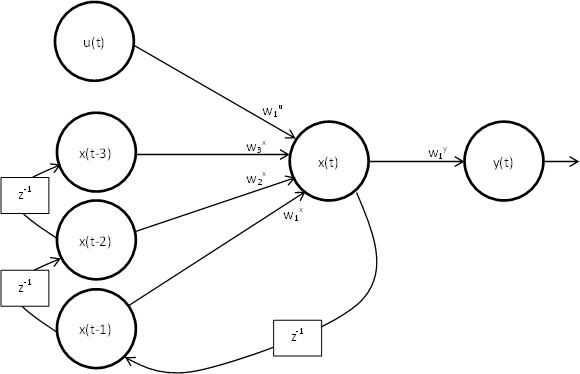
\includegraphics[height=7cm]{architektur2.png}
	\caption{Architektur}
	\label{arche}
\end{figure}

Abbildung \ref{arche} zeigt eine Architektur mit 
\begin{itemize}
	\item einem Inputneuron $u(t)$,
	\item einem verdeckten Neuron $x(t)$,
	\item einem Outputneuron $y(t)$
	\item und drei Kontextneuronen $x(t-1), x(t-2), x(t-3)$
\end{itemize}
mit den dazugeh�rigen Gewichten. Wobei $w_1^u$ das Gewicht der Verbindung vom Inputneuron zum verdeckten Neuron, $w_i^x$, $1 \leq i \leq 3$, die Gewichte von der Kontextschicht zum verdeckten Neuron und $w_1^y$ das Gewicht vom verdeckten Neuron zum Outputneuron darstellen. $z^{-1}$ stellt den Shiftoperator dar, welcher den Wert der Verbindung um einen Zeitschitt verz�gert. Weiters wird als Lernparameter $\eta = 0,7$ und als Aktivierungsfunktion die Sigmoide (Abbildung \ref{sigmoid}) verwendet:
$$\varphi(x) = \frac{1}{1+e^{-x}}$$
\begin{figure}[H]
	\centering
	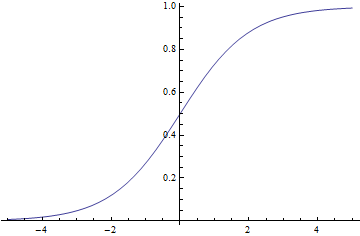
\includegraphics[height=6cm]{sigmoid.png}
	\caption{Sigmoide}
	\label{sigmoid}
\end{figure}

Dieses Netz kann man nun mit dem dynamischen Backpropagation Algorithmus sehr erfolgreich trainieren. Dazu werden 100 Input- und Outputwerte verwendet und es sind folgende Berechnungen pro Zeitschitt n�tig:
\begin{align*}
	v(t) &= w_1^x x(t-1) + w_2^x x(t-2) + w_3^x x(t-3) + w_1^u u(t) \\
	x(t) &= \varphi(v) \\
	y(t) &= w_1^y x(t)
\end{align*}
\begin{align*}
	w_1^u(t) &= w_1^u(t-1) - \eta (y_d(t)-y(t)) w_1^y(t-1) \varphi'(u(t)) \\
	w_1^x(t) &= w_1^x(t-1) - \eta (y_d(t)-y(t)) w_1^y(t-1) \frac{\partial x(t)}{\partial w_1^x(t-1)} \\
	w_2^x(t) &= w_2^x(t-1) - \eta (y_d(t)-y(t)) w_1^y(t-1) \frac{\partial x(t)}{\partial w_2^x(t-1)} \\
	w_3^x(t) &= w_3^x(t-1) - \eta (y_d(t)-y(t)) w_1^y(t-1) \frac{\partial x(t)}{\partial w_3^x(t-1)} \\
	w_1^y(t) &= w_1^y(t-1) - \eta (y_d(t)-y(t)) x(t)
\end{align*}

Ein so trainiertes Elman Netz liefert zum obigen Input-Output Model und nach 100 Epochen folgendes Ergebnis (Abbildung \ref{result1}), wobei die blaue Linie das anzun�hernde Input-Output Model und die violetten Punkte den Netzoutput darstellen.
\begin{figure}[H]
	\centering
	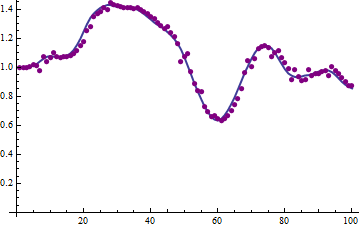
\includegraphics[height=7cm]{Plot1.png}
	\caption{System Identification}
	\label{result1}
\end{figure}

Zu beachten ist, dass durch die Wahl einer anderen Architektur oder bei einem zu niedrig gew�hlten Lernparameter die Ergebnisse trotz dynamischer Backpropagation abweichen k�nnen. Dies zeigt Abbildung \ref{result2}.
\begin{figure}[H]
	\centering
	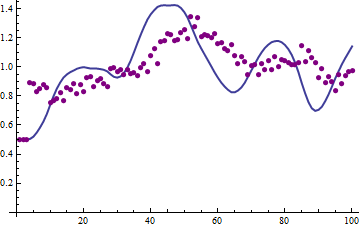
\includegraphics[height=6cm]{Plot2.png}
	\caption{Fehlerdarstellung}
	\label{result2}
\end{figure}
